\documentclass[12pt,a4paper]{article}

% --- Paquetes ---
\usepackage[utf8]{inputenc}
\usepackage[spanish]{babel}
\usepackage[margin=2.5cm]{geometry}
\usepackage{graphicx}
\usepackage{xcolor}
\usepackage{hyperref}
\usepackage{enumitem}

% --- Colores basados en styles.css ---
\definecolor{brandColor}{HTML}{C2410C} 
\definecolor{brandDark}{HTML}{7C2D12}  
\definecolor{ringColor}{HTML}{0F766E}  
\definecolor{bgMain}{HTML}{FFFAF2}     

\hypersetup{
    colorlinks=true,
    linkcolor=brandDark,
    urlcolor=brandColor
}

% --- Portada ---
\title{
    \vspace{2cm}
    \textbf{Memoria Técnica: Proyecto Sabores de Barrio}\\
    \large EPD 2: Diseño de Interfaces Avanzado - Bootstrap 5.3\\
    \vspace{0.5cm}
    \normalsize Tecnologías Avanzadas de Desarrollo
}
\author{\textbf{Oleksandr B. Baranets}}
\date{\today}

\begin{document}

\maketitle

\begin{center}
    \vspace{1cm}
    \textbf{Enlace GitHub Pages:} \\
    \url{https://superv1s0r.github.io/tda_epd2/}
    \vspace{1cm}
    \textbf{Enlace a repositorio}
    \url{https://github.com/superv1s0r/tda_epd2/}
\end{center}

\newpage
% --- Índice de contenidos ---
\tableofcontents 
\newpage

\section{Uso y Finalidad del Proyecto}
Sabores de Barrio es una guía interactiva de mercados y cocina local en Sevilla. El proyecto busca fomentar el consumo de proximidad y la cultura culinaria tradicional, evitando el uso de texto falso conforme a los requisitos.

\section{Componentes de Bootstrap 5.3 Empleados}
Se han integrado más de 10 componentes distintos de la versión 5.3.3:
\begin{itemize}
    \item \textbf{Navbar y Offcanvas:} Para una navegación adaptable.
    \item \textbf{Carousel:} Galería dinámica de imágenes en la cabecera.
    \item \textbf{Cards:} Para la presentación visual de las rutas gastronómicas.
    \item \textbf{Progress Bars:} Visualización de métricas de impacto local.
    \item \textbf{Accordion:} Sección de preguntas frecuentes optimizada.
    \item \textbf{Forms y Validation:} Formulario de reserva con validación de datos.
    \item \textbf{Toasts:} Avisos de confirmación tras el envío del formulario.
\end{itemize}

\section{Diseño Visual y Tipografía}
\subsection{Paleta de Colores}
Basado en el archivo \texttt{styles.css}, se utilizan tonos tierra y orgánicos:
\begin{itemize}
    \item \textbf{Primario:} \texttt{\#C2410C} (Naranja marca).
    \item \textbf{Acento:} \texttt{\#0F766E} (Verde anillo para barras de progreso).
    \item \textbf{Fondo:} \texttt{\#FFFAF2} (Crema principal).
\end{itemize}

\subsection{Fuentes (Google Fonts)}
Se han seleccionado fuentes que combinan modernidad y tradición:
\begin{itemize}
    \item \textbf{Bricolage Grotesque:} Para el cuerpo de texto y elementos de UI.
    \item \textbf{Newsreader:} Para encabezados, aportando un estilo editorial.
\end{itemize}

\section{Lógica de Cliente (JavaScript)}
El archivo \texttt{main.js} gestiona la interacción del formulario de reserva. Implementa la validación de campos obligatorios y activa el componente Toast de Bootstrap una vez que los datos son correctos.

\section{Diseño Adaptativo: Smartphone}
En pantallas pequeñas, los elementos de navegación se agrupan en un menú lateral \textbf{Offcanvas} para priorizar el contenido visual.
\begin{figure}[h]
    \centering
    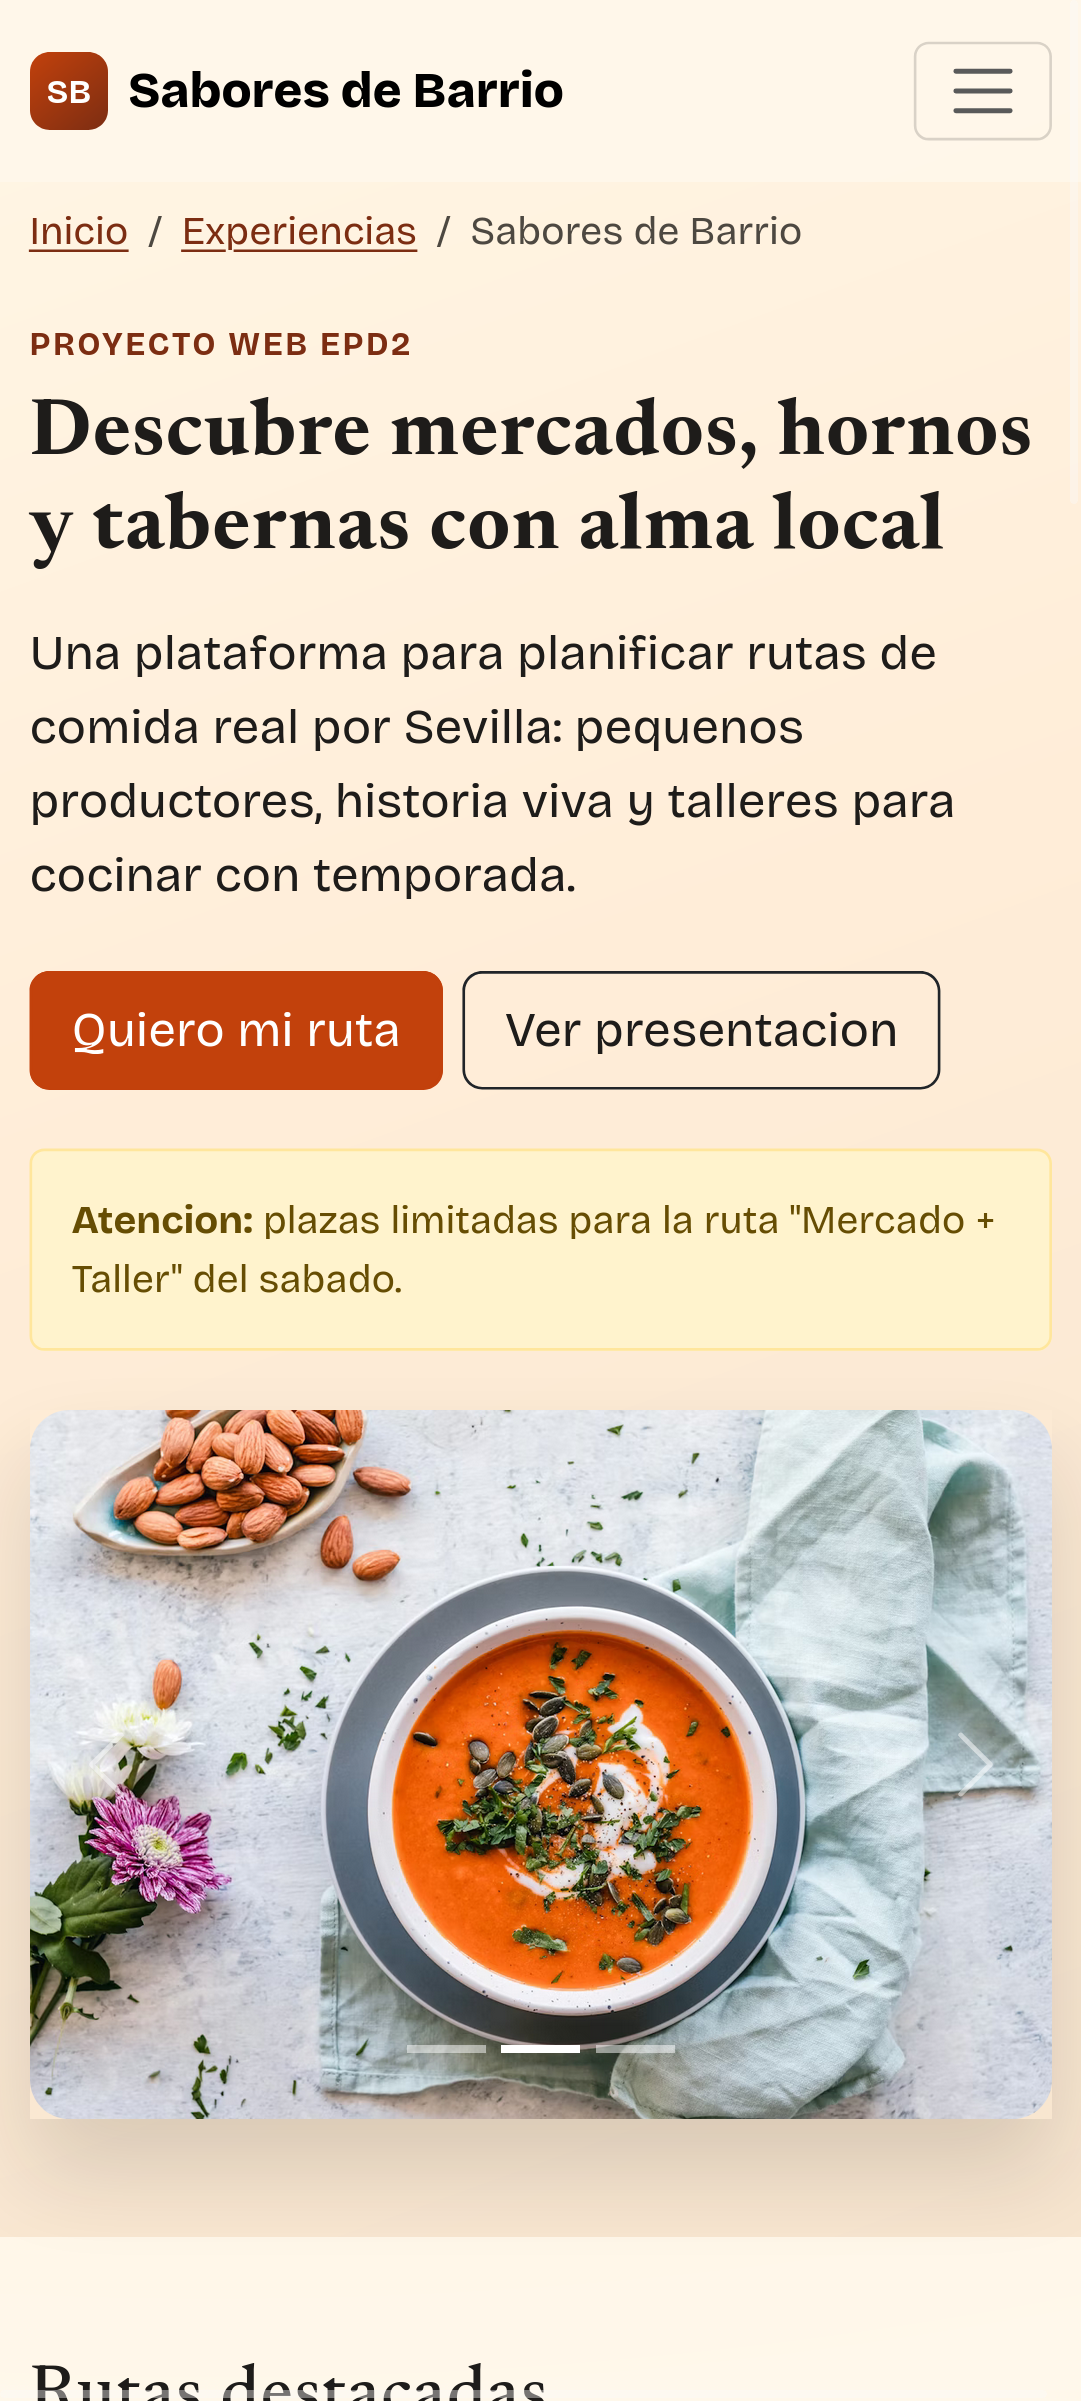
\includegraphics[width=0.35\textwidth]{movil.png}
    \caption{Interfaz optimizada para dispositivos móviles.}
\end{figure}
\newpage
\section{Diseño Adaptativo: Tablet (iPad)}
El sistema de rejilla de Bootstrap permite que las tarjetas de rutas se reorganicen en columnas dobles, aprovechando mejor el ancho de pantalla de una tablet.
\begin{figure}[h]
    \centering
    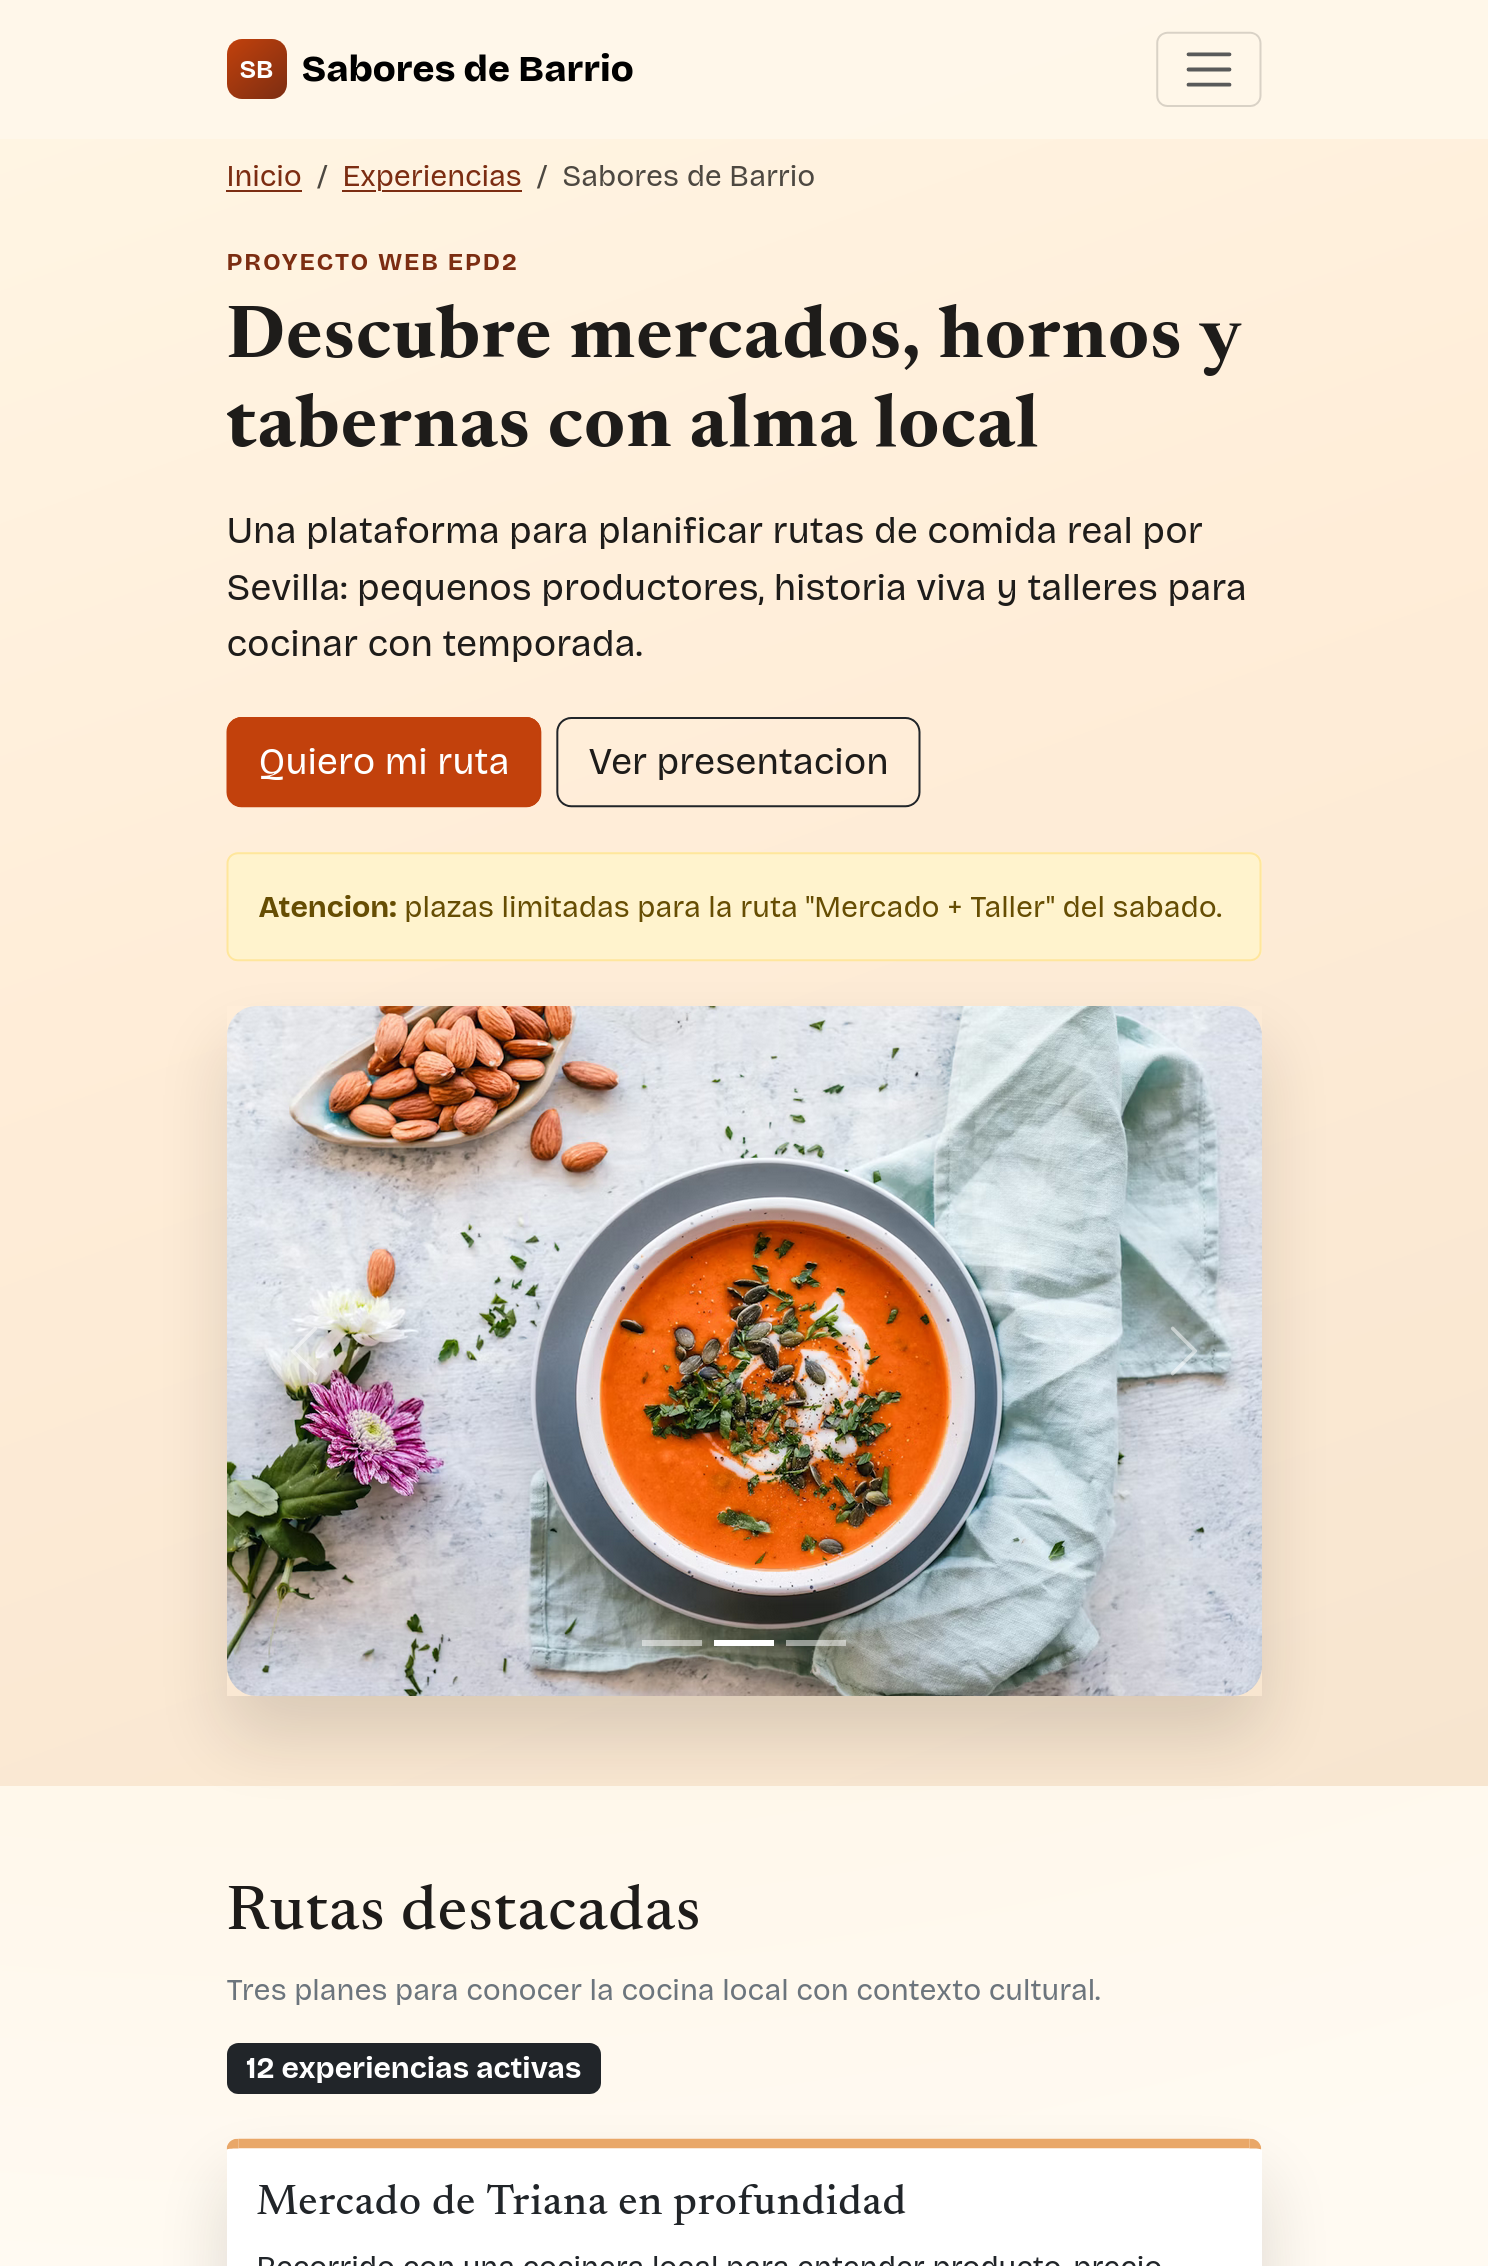
\includegraphics[width=0.7\textwidth]{ipad.png}
    \caption{Distribución de contenido en iPad.}
\end{figure}
\newpage

\section{Diseño Adaptativo: TV HD}
En pantallas de gran formato, se aplican efectos de desenfoque de fondo (\textit{backdrop-filter}) y degradados complejos definidos en el CSS para una experiencia inmersiva.
\begin{figure}[h]
    \centering
    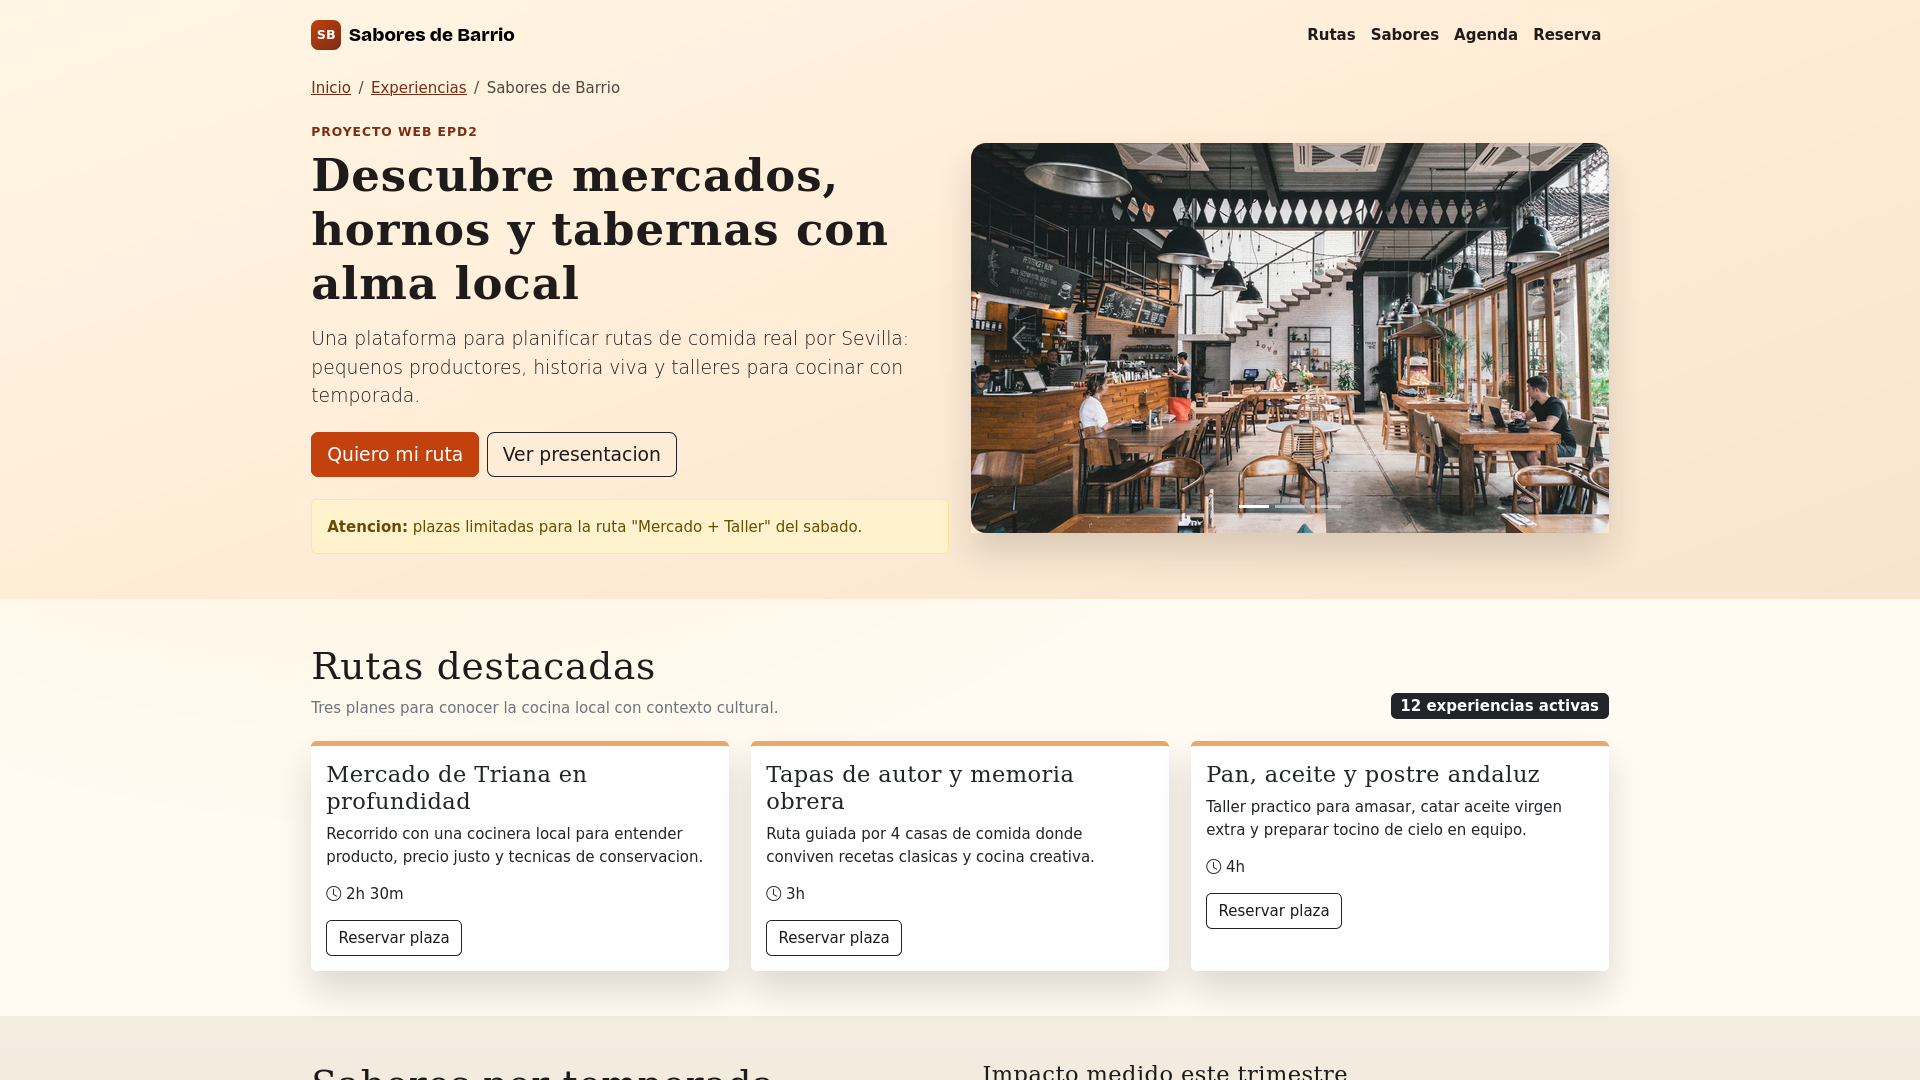
\includegraphics[width=0.9\textwidth]{tv_hd.png}
    \caption{Visualización en alta resolución.}
\end{figure}


\newpage

\section{Accesibilidad (WCAG)}
El proyecto cumple con normativas de accesibilidad para asegurar la inclusión:
\begin{itemize}
    \item \textbf{Skip Link:} Permite saltar al contenido principal mediante teclado.
    \item \textbf{Roles ARIA:} Uso de atributos \texttt{aria-label} y \texttt{aria-live} para lectores de pantalla.
    \item \textbf{Reducción de movimiento:} Soporte para usuarios con sensibilidad mediante \texttt{prefers-reduced-motion}.
\end{itemize}

\section{Problemas y Soluciones}
\begin{itemize}
    \item \textbf{Problema:} La validación del formulario no se limpiaba tras el reinicio.
    \item \textbf{Solución:} Se programó la eliminación manual de la clase \texttt{was-validated} en el script \texttt{main.js}.
\end{itemize}

\end{document}